% Options for packages loaded elsewhere
\PassOptionsToPackage{unicode}{hyperref}
\PassOptionsToPackage{hyphens}{url}
%
\documentclass[
]{article}
\usepackage{amsmath,amssymb}
\usepackage{lmodern}
\usepackage{ifxetex,ifluatex}
\ifnum 0\ifxetex 1\fi\ifluatex 1\fi=0 % if pdftex
  \usepackage[T1]{fontenc}
  \usepackage[utf8]{inputenc}
  \usepackage{textcomp} % provide euro and other symbols
\else % if luatex or xetex
  \usepackage{unicode-math}
  \defaultfontfeatures{Scale=MatchLowercase}
  \defaultfontfeatures[\rmfamily]{Ligatures=TeX,Scale=1}
\fi
% Use upquote if available, for straight quotes in verbatim environments
\IfFileExists{upquote.sty}{\usepackage{upquote}}{}
\IfFileExists{microtype.sty}{% use microtype if available
  \usepackage[]{microtype}
  \UseMicrotypeSet[protrusion]{basicmath} % disable protrusion for tt fonts
}{}
\makeatletter
\@ifundefined{KOMAClassName}{% if non-KOMA class
  \IfFileExists{parskip.sty}{%
    \usepackage{parskip}
  }{% else
    \setlength{\parindent}{0pt}
    \setlength{\parskip}{6pt plus 2pt minus 1pt}}
}{% if KOMA class
  \KOMAoptions{parskip=half}}
\makeatother
\usepackage{xcolor}
\IfFileExists{xurl.sty}{\usepackage{xurl}}{} % add URL line breaks if available
\IfFileExists{bookmark.sty}{\usepackage{bookmark}}{\usepackage{hyperref}}
\hypersetup{
  pdftitle={Econometriscs assignment},
  pdfauthor={Heidi Marie Rolfsnes and Ann Elisabeth Jacobsen},
  hidelinks,
  pdfcreator={LaTeX via pandoc}}
\urlstyle{same} % disable monospaced font for URLs
\usepackage[margin=1in]{geometry}
\usepackage{color}
\usepackage{fancyvrb}
\newcommand{\VerbBar}{|}
\newcommand{\VERB}{\Verb[commandchars=\\\{\}]}
\DefineVerbatimEnvironment{Highlighting}{Verbatim}{commandchars=\\\{\}}
% Add ',fontsize=\small' for more characters per line
\usepackage{framed}
\definecolor{shadecolor}{RGB}{248,248,248}
\newenvironment{Shaded}{\begin{snugshade}}{\end{snugshade}}
\newcommand{\AlertTok}[1]{\textcolor[rgb]{0.94,0.16,0.16}{#1}}
\newcommand{\AnnotationTok}[1]{\textcolor[rgb]{0.56,0.35,0.01}{\textbf{\textit{#1}}}}
\newcommand{\AttributeTok}[1]{\textcolor[rgb]{0.77,0.63,0.00}{#1}}
\newcommand{\BaseNTok}[1]{\textcolor[rgb]{0.00,0.00,0.81}{#1}}
\newcommand{\BuiltInTok}[1]{#1}
\newcommand{\CharTok}[1]{\textcolor[rgb]{0.31,0.60,0.02}{#1}}
\newcommand{\CommentTok}[1]{\textcolor[rgb]{0.56,0.35,0.01}{\textit{#1}}}
\newcommand{\CommentVarTok}[1]{\textcolor[rgb]{0.56,0.35,0.01}{\textbf{\textit{#1}}}}
\newcommand{\ConstantTok}[1]{\textcolor[rgb]{0.00,0.00,0.00}{#1}}
\newcommand{\ControlFlowTok}[1]{\textcolor[rgb]{0.13,0.29,0.53}{\textbf{#1}}}
\newcommand{\DataTypeTok}[1]{\textcolor[rgb]{0.13,0.29,0.53}{#1}}
\newcommand{\DecValTok}[1]{\textcolor[rgb]{0.00,0.00,0.81}{#1}}
\newcommand{\DocumentationTok}[1]{\textcolor[rgb]{0.56,0.35,0.01}{\textbf{\textit{#1}}}}
\newcommand{\ErrorTok}[1]{\textcolor[rgb]{0.64,0.00,0.00}{\textbf{#1}}}
\newcommand{\ExtensionTok}[1]{#1}
\newcommand{\FloatTok}[1]{\textcolor[rgb]{0.00,0.00,0.81}{#1}}
\newcommand{\FunctionTok}[1]{\textcolor[rgb]{0.00,0.00,0.00}{#1}}
\newcommand{\ImportTok}[1]{#1}
\newcommand{\InformationTok}[1]{\textcolor[rgb]{0.56,0.35,0.01}{\textbf{\textit{#1}}}}
\newcommand{\KeywordTok}[1]{\textcolor[rgb]{0.13,0.29,0.53}{\textbf{#1}}}
\newcommand{\NormalTok}[1]{#1}
\newcommand{\OperatorTok}[1]{\textcolor[rgb]{0.81,0.36,0.00}{\textbf{#1}}}
\newcommand{\OtherTok}[1]{\textcolor[rgb]{0.56,0.35,0.01}{#1}}
\newcommand{\PreprocessorTok}[1]{\textcolor[rgb]{0.56,0.35,0.01}{\textit{#1}}}
\newcommand{\RegionMarkerTok}[1]{#1}
\newcommand{\SpecialCharTok}[1]{\textcolor[rgb]{0.00,0.00,0.00}{#1}}
\newcommand{\SpecialStringTok}[1]{\textcolor[rgb]{0.31,0.60,0.02}{#1}}
\newcommand{\StringTok}[1]{\textcolor[rgb]{0.31,0.60,0.02}{#1}}
\newcommand{\VariableTok}[1]{\textcolor[rgb]{0.00,0.00,0.00}{#1}}
\newcommand{\VerbatimStringTok}[1]{\textcolor[rgb]{0.31,0.60,0.02}{#1}}
\newcommand{\WarningTok}[1]{\textcolor[rgb]{0.56,0.35,0.01}{\textbf{\textit{#1}}}}
\usepackage{graphicx}
\makeatletter
\def\maxwidth{\ifdim\Gin@nat@width>\linewidth\linewidth\else\Gin@nat@width\fi}
\def\maxheight{\ifdim\Gin@nat@height>\textheight\textheight\else\Gin@nat@height\fi}
\makeatother
% Scale images if necessary, so that they will not overflow the page
% margins by default, and it is still possible to overwrite the defaults
% using explicit options in \includegraphics[width, height, ...]{}
\setkeys{Gin}{width=\maxwidth,height=\maxheight,keepaspectratio}
% Set default figure placement to htbp
\makeatletter
\def\fps@figure{htbp}
\makeatother
\setlength{\emergencystretch}{3em} % prevent overfull lines
\providecommand{\tightlist}{%
  \setlength{\itemsep}{0pt}\setlength{\parskip}{0pt}}
\setcounter{secnumdepth}{-\maxdimen} % remove section numbering
\usepackage{booktabs}
\usepackage{longtable}
\usepackage{array}
\usepackage{multirow}
\usepackage{wrapfig}
\usepackage{float}
\usepackage{colortbl}
\usepackage{pdflscape}
\usepackage{tabu}
\usepackage{threeparttable}
\usepackage{threeparttablex}
\usepackage[normalem]{ulem}
\usepackage{makecell}
\usepackage{xcolor}
\ifluatex
  \usepackage{selnolig}  % disable illegal ligatures
\fi

\title{Econometriscs assignment}
\author{Heidi Marie Rolfsnes and Ann Elisabeth Jacobsen}
\date{}

\begin{document}
\maketitle

\begin{verbatim}
## Warning in !is.null(rmarkdown::metadata$output) && rmarkdown::metadata$output
## %in% : 'length(x) = 3 > 1' in coercion to 'logical(1)'
\end{verbatim}

\hypertarget{introduction}{%
\subsection{Introduction}\label{introduction}}

In the subject MSB104 econometrics, this year we will hand in an
assignment divided into four assignments throughout the semester. The
assignments must be written and calculated in the software R. We are
group one and the countries that will be representing in our assignment
is: Denmark, France, Hungary, Portugal and Slovakia.

\hypertarget{assignment-1}{%
\subsection{Assignment 1}\label{assignment-1}}

In this assignment we are going to download two dataset from Eurostat.
The data contains GDP (nama\_10r\_3gdp) and populations
(demo\_r\_pjanaggr3,pi) for countries over the last 20 years, on a NUTS3
level. When we have all the information we need from the dataset, we are
going to calculate the GDP per capita and describe the data by using the
meta data description from Eurostat.

In the second part of this assignment we will use our data to calculate
the population watertight GDP Ginie coefficients for the European NUTS2
(j) level and describe our new data. Then we are going to plot the
distribution of Ginie coefficients In the end of the first assignment we
will discuss if there are noteworthy outliers.

\hypertarget{dataset}{%
\subsubsection{Dataset}\label{dataset}}

The dataset ``Nama\_10r\_3gdp'' contains GDP for many countries
including our five countries on a NUTS3 level. The datset is structured
in eight columns and each column present different data values. We are
looking for the GDP values and it emerges from the column
``OBS\_VALUE''. The column ``GEO'' tells us which geographical region
the value belongs to. There is also a column for year named
``TIME\_PERIOD''. We are going to work with these three columns and will
start with rename the names of the columns. There are different types of
GDP values and the unit is stored in a column named ``UNIT''. We have
chosen to use values where unit is MIO\_EUR. This unit represents the
GDP value in million Euros.

The dataset Demo\_r\_pjanaggr3 contains population data on nuts3 level
for our five countries. The two datasets we obtained from Eurostat are
quite similar and the population dataset also contains Time\_period,
Obs\_value and geo. We will rename the names of the columns we will use,
in the same way as we did in the GDP dataset.

We made a new data set called BNP2 (Norwegian word for GDP and a
number). In this data set we will gather the information we need from
the other two data sets and compile it into one data set.

\begin{table}

\caption{\label{tab:unnamed-chunk-1}Summary Statistics}
\centering
\begin{tabular}[t]{llllllll}
\toprule
Variable & N & Mean & Std. Dev. & Min & Pctl. 25 & Pctl. 75 & Max\\
\midrule
unit & 3380 &  &  &  &  &  & \\
... MIO_EUR & 3380 & 100% &  &  &  &  & \\
Year & 3380 & 2010.5 & 5.767 & 2001 & 2005.75 & 2015.25 & 2020\\
GDP & 3380 & 15374.633 & 22789.799 & 0 & 3739.325 & 18233.838 & 251623.58\\
Population & 3057 & 587529.832 & 477585.739 & 39583 & 263091 & 709496 & 2863272\\
\bottomrule
\end{tabular}
\end{table}

\hypertarget{gdp-per-capita}{%
\subsubsection{GDP per Capita}\label{gdp-per-capita}}

To calculate GDP per capita, we have taken GDP and divided it by the
population. Finally, we have multiplied by one million so that it is
represented correctly in Euros, also like it is in the unit.

We have divided the countries into NUTS3 levels. To get the result by
country, we made a summary of GDP per capita on each country. By
creating such a summary for each country, we can get an overview of
whether there are major inequality within the various regions. If we
find such deviations, we can choose to remove some of our regions in
order not to have large inequalities.

Briefly about what we can find in the summary. We find the min and max.
i.e.~the smallest and the highest GDP per capita for the country. We
also find 1st quartile and 3rd quartile. The first quartile is the
observation between the median and the lowest value, and looks at the
25\% lowest values from the 75\% highest. The median looks at the value
that is observed the most times in the middle of the observations. The
third quartile is then, naturally enough, the value between the median
and the highest value.We will also look at mean which tell us what the
average observation for all regions is.

Lets start with Denmark and then take the countries alphabetically.

\#\#Denmark

Denmark are missing observations for some of the years, so there are
less data to be collected about them. Denmark is also a small country so
there are not that many NUTS2 regions.

\textbf{Country level}

\begin{Shaded}
\begin{Highlighting}[]
    \FunctionTok{summarise}\NormalTok{(DK, }\AttributeTok{GDP\_per\_Capita =} \FunctionTok{mean}\NormalTok{(Per\_capita))}
\end{Highlighting}
\end{Shaded}

\begin{verbatim}
##   GDP_per_Capita
## 1       44208.62
\end{verbatim}

\begin{Shaded}
\begin{Highlighting}[]
\FunctionTok{summary}\NormalTok{(DK)}
\end{Highlighting}
\end{Shaded}

\begin{verbatim}
##       Year        Regio_id           Per_capita      Population    
##  Min.   :2007   Length:154         Min.   :27606   Min.   : 39583  
##  1st Qu.:2010   Class :character   1st Qu.:35172   1st Qu.:429180  
##  Median :2014   Mode  :character   Median :40004   Median :528002  
##  Mean   :2014                      Mean   :44209   Mean   :512116  
##  3rd Qu.:2017                      3rd Qu.:48033   3rd Qu.:675962  
##  Max.   :2020                      Max.   :86083   Max.   :897129
\end{verbatim}

\textbf{Regions in Denmark}

\begin{Shaded}
\begin{Highlighting}[]
\NormalTok{BNP2 }\SpecialCharTok{\%\textgreater{}\%}
  \FunctionTok{filter}\NormalTok{(}\FunctionTok{grepl}\NormalTok{(}\StringTok{"DK..."}\NormalTok{, Regio\_id)) }\SpecialCharTok{\%\textgreater{}\%}
  \FunctionTok{select}\NormalTok{(}\SpecialCharTok{{-}}\NormalTok{Regio\_id) }\SpecialCharTok{\%\textgreater{}\%}
\NormalTok{  vtable}\SpecialCharTok{::}\FunctionTok{st}\NormalTok{(.)}
\end{Highlighting}
\end{Shaded}

\begin{table}

\caption{\label{tab:unnamed-chunk-3}Summary Statistics}
\centering
\begin{tabular}[t]{llllllll}
\toprule
Variable & N & Mean & Std. Dev. & Min & Pctl. 25 & Pctl. 75 & Max\\
\midrule
unit & 154 &  &  &  &  &  & \\
... MIO_EUR & 154 & 100% &  &  &  &  & \\
Year & 154 & 2013.5 & 4.044 & 2007 & 2010 & 2017 & 2020\\
GDP & 154 & 23806.301 & 13688.78 & 1229.95 & 16587.845 & 33419.845 & 59302.48\\
Population & 154 & 512115.844 & 218524.351 & 39583 & 429179.5 & 675961.75 & 897129\\
\addlinespace
Per_capita & 154 & 44208.617 & 13479.231 & 27605.859 & 35172.249 & 48033.058 & 86082.754\\
\bottomrule
\end{tabular}
\end{table}

To make it even more specific, we can choose to look at a specific year,
and find out which regions are most whealty that year and which regions
come out poorly that exact year. We choose 2020, which is the last year
that is included in the calculation, and therefore closest to 2022,
which we are in today. We have also chosen to look at the 5 richest and
the 5 poorest regions to see if there are major differences. We will do
the same with all of our five countries.

\begin{Shaded}
\begin{Highlighting}[]
\NormalTok{GDPDK }\OtherTok{\textless{}{-}}\NormalTok{ BNP2}\SpecialCharTok{\%\textgreater{}\%}
  \FunctionTok{filter}\NormalTok{(}\FunctionTok{grepl}\NormalTok{(}\StringTok{"DK..."}\NormalTok{, Regio\_id)) }\SpecialCharTok{\%\textgreater{}\%}
  \FunctionTok{filter}\NormalTok{(Year}\SpecialCharTok{==}\DecValTok{2020}\NormalTok{) }\SpecialCharTok{\%\textgreater{}\%}
  \FunctionTok{select}\NormalTok{(Regio\_id, Per\_capita)}
\FunctionTok{slice\_max}\NormalTok{(GDPDK, Per\_capita, }\AttributeTok{n=}\DecValTok{5}\NormalTok{)}
\end{Highlighting}
\end{Shaded}

\begin{verbatim}
##   Regio_id Per_capita
## 1    DK012   86082.75
## 2    DK011   74676.22
## 3    DK032   52121.61
## 4    DK041   52052.00
## 5    DK042   47918.09
\end{verbatim}

\begin{Shaded}
\begin{Highlighting}[]
\FunctionTok{slice\_min}\NormalTok{(GDPDK, Per\_capita, }\AttributeTok{n=}\DecValTok{5}\NormalTok{)}
\end{Highlighting}
\end{Shaded}

\begin{verbatim}
##   Regio_id Per_capita
## 1    DK022   37529.24
## 2    DK014   37811.94
## 3    DK021   37963.88
## 4    DK031   40611.19
## 5    DK050   44623.48
\end{verbatim}

As we can see above Denmark is\ldots{}

\#\#France

France is a large country, it has over a hundred NUTS3 regions.

\begin{Shaded}
\begin{Highlighting}[]
\FunctionTok{summary}\NormalTok{(FR)}
\end{Highlighting}
\end{Shaded}

\begin{verbatim}
##       Year        Regio_id           Per_capita       Population     
##  Min.   :2002   Length:1630        Min.   :  8292   Min.   :  74857  
##  1st Qu.:2006   Class :character   1st Qu.: 22050   1st Qu.: 279223  
##  Median :2011   Mode  :character   Median : 24476   Median : 526667  
##  Mean   :2011                      Mean   : 26869   Mean   : 642083  
##  3rd Qu.:2016                      3rd Qu.: 28270   3rd Qu.: 833425  
##  Max.   :2020                      Max.   :116235   Max.   :2249975
\end{verbatim}

In the summary of France there are a hug differense in min and max. this
is because France has colonies in other countries that are counted.
These colonies are located in Africa and South America which have a
negative effect on the overall GDP of France. For further research these
countries should be removed from the data set.

\textbf{Country level}

\begin{Shaded}
\begin{Highlighting}[]
    \FunctionTok{summarise}\NormalTok{(FR, }\AttributeTok{GDP\_per\_Capita =} \FunctionTok{mean}\NormalTok{(Per\_capita))}
\end{Highlighting}
\end{Shaded}

\begin{verbatim}
## `summarise()` has grouped output by 'Regio_id'. You can override using the
## `.groups` argument.
\end{verbatim}

\begin{verbatim}
## # A tibble: 1,630 x 3
## # Groups:   Regio_id [87]
##    Regio_id  Year GDP_per_Capita
##    <chr>    <dbl>          <dbl>
##  1 FR101     2002         75369.
##  2 FR101     2003         75357.
##  3 FR101     2004         76586.
##  4 FR101     2005         79258.
##  5 FR101     2006         80305.
##  6 FR101     2007         85155.
##  7 FR101     2008         85583.
##  8 FR101     2009         81539.
##  9 FR101     2010         87627.
## 10 FR101     2011         88674.
## # ... with 1,620 more rows
\end{verbatim}

\begin{Shaded}
\begin{Highlighting}[]
\FunctionTok{summary}\NormalTok{(FR1)}
\end{Highlighting}
\end{Shaded}

\begin{verbatim}
##       Year        Regio_id           Per_capita       Population     
##  Min.   :2002   Length:1558        Min.   : 16619   Min.   :  74857  
##  1st Qu.:2006   Class :character   1st Qu.: 22286   1st Qu.: 281078  
##  Median :2011   Mode  :character   Median : 24670   Median : 534055  
##  Mean   :2011                      Mean   : 27290   Mean   : 650912  
##  3rd Qu.:2016                      3rd Qu.: 28532   3rd Qu.: 899310  
##  Max.   :2020                      Max.   :116235   Max.   :2249975
\end{verbatim}

\textbf{Regions in France}

\begin{Shaded}
\begin{Highlighting}[]
\NormalTok{BNP2 }\SpecialCharTok{\%\textgreater{}\%}
  \FunctionTok{filter}\NormalTok{(}\FunctionTok{grepl}\NormalTok{(}\StringTok{"FR..."}\NormalTok{, Regio\_id)) }\SpecialCharTok{\%\textgreater{}\%}
  \FunctionTok{select}\NormalTok{(}\SpecialCharTok{{-}}\NormalTok{Regio\_id) }\SpecialCharTok{\%\textgreater{}\%}
\NormalTok{  vtable}\SpecialCharTok{::}\FunctionTok{st}\NormalTok{(.)}
\end{Highlighting}
\end{Shaded}

\begin{table}

\caption{\label{tab:unnamed-chunk-6}Summary Statistics}
\centering
\begin{tabular}[t]{llllllll}
\toprule
Variable & N & Mean & Std. Dev. & Min & Pctl. 25 & Pctl. 75 & Max\\
\midrule
unit & 1896 &  &  &  &  &  & \\
... MIO_EUR & 1896 & 100% &  &  &  &  & \\
Year & 1896 & 2011.045 & 5.484 & 2002 & 2006 & 2016 & 2020\\
GDP & 1896 & 20320.969 & 27244.934 & 1378.33 & 6508.568 & 21478.63 & 251623.58\\
Population & 1896 & 647061.273 & 491521.428 & 74857 & 291513 & 821240 & 2606234\\
\addlinespace
Per_capita & 1896 & 26772.041 & 10672.979 & 8291.874 & 22234.94 & 28372.722 & 116235.12\\
\bottomrule
\end{tabular}
\end{table}

\begin{Shaded}
\begin{Highlighting}[]
\NormalTok{GDPFR }\OtherTok{\textless{}{-}}\NormalTok{ BNP2}\SpecialCharTok{\%\textgreater{}\%}
  \FunctionTok{filter}\NormalTok{(}\FunctionTok{grepl}\NormalTok{(}\StringTok{"FR..."}\NormalTok{, Regio\_id)) }\SpecialCharTok{\%\textgreater{}\%}
  \FunctionTok{filter}\NormalTok{(Year}\SpecialCharTok{==}\DecValTok{2020}\NormalTok{) }\SpecialCharTok{\%\textgreater{}\%}
  \FunctionTok{select}\NormalTok{(Regio\_id, Per\_capita)}
\FunctionTok{slice\_max}\NormalTok{(GDPFR, Per\_capita, }\AttributeTok{n=}\DecValTok{5}\NormalTok{)}
\end{Highlighting}
\end{Shaded}

\begin{verbatim}
##   Regio_id Per_capita
## 1    FR101  109033.47
## 2    FR105  107512.18
## 3    FRK26   47312.59
## 4    FR104   41823.82
## 5    FRJ23   39294.57
\end{verbatim}

\begin{Shaded}
\begin{Highlighting}[]
\FunctionTok{slice\_min}\NormalTok{(GDPFR, Per\_capita, }\AttributeTok{n=}\DecValTok{5}\NormalTok{)}
\end{Highlighting}
\end{Shaded}

\begin{verbatim}
##   Regio_id Per_capita
## 1    FRY50   9884.342
## 2    FRY30  15103.129
## 3    FRI22  20166.155
## 4    FRJ21  20941.853
## 5    FRC23  20986.626
\end{verbatim}

As we can see above France is\ldots{}

\#\#Hungary

\textbf{Country level}

\begin{Shaded}
\begin{Highlighting}[]
    \FunctionTok{summarise}\NormalTok{(HU, }\AttributeTok{GDP\_per\_Capita =} \FunctionTok{mean}\NormalTok{(Per\_capita))}
\end{Highlighting}
\end{Shaded}

\begin{verbatim}
## `summarise()` has grouped output by 'Regio_id'. You can override using the
## `.groups` argument.
\end{verbatim}

\begin{verbatim}
## # A tibble: 380 x 3
## # Groups:   Regio_id [20]
##    Regio_id  Year GDP_per_Capita
##    <chr>    <dbl>          <dbl>
##  1 HU110     2002         14449.
##  2 HU110     2003         15013.
##  3 HU110     2004         17088.
##  4 HU110     2005         19097.
##  5 HU110     2006         19739.
##  6 HU110     2007         21939.
##  7 HU110     2008         23699.
##  8 HU110     2009         21452.
##  9 HU110     2010         21946.
## 10 HU110     2011         22268.
## # ... with 370 more rows
\end{verbatim}

\begin{Shaded}
\begin{Highlighting}[]
\FunctionTok{summary}\NormalTok{(HU)}
\end{Highlighting}
\end{Shaded}

\begin{verbatim}
##       Year        Regio_id           Per_capita      Population     
##  Min.   :2002   Length:380         Min.   : 3773   Min.   : 188092  
##  1st Qu.:2006   Class :character   1st Qu.: 6330   1st Qu.: 305718  
##  Median :2011   Mode  :character   Median : 7754   Median : 393302  
##  Mean   :2011                      Mean   : 8782   Mean   : 498087  
##  3rd Qu.:2016                      3rd Qu.: 9907   3rd Qu.: 536534  
##  Max.   :2020                      Max.   :31013   Max.   :1759407
\end{verbatim}

\textbf{Regions in Hungary}

\begin{Shaded}
\begin{Highlighting}[]
\NormalTok{BNP2 }\SpecialCharTok{\%\textgreater{}\%}
  \FunctionTok{filter}\NormalTok{(}\FunctionTok{grepl}\NormalTok{(}\StringTok{"HU..."}\NormalTok{, Regio\_id)) }\SpecialCharTok{\%\textgreater{}\%}
  \FunctionTok{select}\NormalTok{(}\SpecialCharTok{{-}}\NormalTok{Regio\_id) }\SpecialCharTok{\%\textgreater{}\%}
\NormalTok{  vtable}\SpecialCharTok{::}\FunctionTok{st}\NormalTok{(.)}
\end{Highlighting}
\end{Shaded}

\begin{table}

\caption{\label{tab:unnamed-chunk-8}Summary Statistics}
\centering
\begin{tabular}[t]{llllllll}
\toprule
Variable & N & Mean & Std. Dev. & Min & Pctl. 25 & Pctl. 75 & Max\\
\midrule
unit & 380 &  &  &  &  &  & \\
... MIO_EUR & 380 & 100% &  &  &  &  & \\
Year & 380 & 2011 & 5.484 & 2002 & 2006 & 2016 & 2020\\
GDP & 380 & 5278.015 & 8149.841 & 832.24 & 2296.778 & 4210.142 & 54343.95\\
Population & 380 & 498086.908 & 354417.845 & 188092 & 305718 & 536534.5 & 1759407\\
\addlinespace
Per_capita & 380 & 8781.693 & 4054.096 & 3772.62 & 6329.585 & 9906.789 & 31013.174\\
\bottomrule
\end{tabular}
\end{table}

\begin{Shaded}
\begin{Highlighting}[]
\NormalTok{GDPHU }\OtherTok{\textless{}{-}}\NormalTok{ BNP2}\SpecialCharTok{\%\textgreater{}\%}
  \FunctionTok{filter}\NormalTok{(}\FunctionTok{grepl}\NormalTok{(}\StringTok{"HU..."}\NormalTok{, Regio\_id)) }\SpecialCharTok{\%\textgreater{}\%}
  \FunctionTok{filter}\NormalTok{(Year}\SpecialCharTok{==}\DecValTok{2020}\NormalTok{) }\SpecialCharTok{\%\textgreater{}\%}
  \FunctionTok{select}\NormalTok{(Regio\_id, Per\_capita)}
\FunctionTok{slice\_max}\NormalTok{(GDPHU, Per\_capita, }\AttributeTok{n=}\DecValTok{5}\NormalTok{)}
\end{Highlighting}
\end{Shaded}

\begin{verbatim}
##   Regio_id Per_capita
## 1    HU110   28814.04
## 2    HU221   15922.99
## 3    HU211   13848.85
## 4    HU212   13465.04
## 5    HU222   12078.56
\end{verbatim}

\begin{Shaded}
\begin{Highlighting}[]
\FunctionTok{slice\_min}\NormalTok{(GDPHU, Per\_capita, }\AttributeTok{n=}\DecValTok{5}\NormalTok{)}
\end{Highlighting}
\end{Shaded}

\begin{verbatim}
##   Regio_id Per_capita
## 1    HU313   6319.408
## 2    HU323   8092.028
## 3    HU332   8289.658
## 4    HU232   9113.019
## 5    HU322   9508.020
\end{verbatim}

As we can see above Hungary is\ldots{}

\hypertarget{portugal}{%
\subsection{Portugal}\label{portugal}}

\textbf{Country level}

\begin{Shaded}
\begin{Highlighting}[]
    \FunctionTok{summarise}\NormalTok{(PT, }\AttributeTok{GDP\_per\_Capita =} \FunctionTok{mean}\NormalTok{(Per\_capita))}
\end{Highlighting}
\end{Shaded}

\begin{verbatim}
##   GDP_per_Capita
## 1       14415.77
\end{verbatim}

\begin{Shaded}
\begin{Highlighting}[]
\FunctionTok{summary}\NormalTok{(PT)}
\end{Highlighting}
\end{Shaded}

\begin{verbatim}
##       Year        Regio_id           Per_capita      Population     
##  Min.   :2002   Length:456         Min.   : 7212   Min.   :  80230  
##  1st Qu.:2006   Class :character   1st Qu.:12125   1st Qu.: 147877  
##  Median :2011   Mode  :character   Median :14045   Median : 248738  
##  Mean   :2011                      Mean   :14416   Mean   : 417150  
##  3rd Qu.:2016                      3rd Qu.:16087   3rd Qu.: 376989  
##  Max.   :2020                      Max.   :27207   Max.   :2863272
\end{verbatim}

\textbf{Regions in Portugal}

\begin{Shaded}
\begin{Highlighting}[]
\NormalTok{BNP2 }\SpecialCharTok{\%\textgreater{}\%}
  \FunctionTok{filter}\NormalTok{(}\FunctionTok{grepl}\NormalTok{(}\StringTok{"PT..."}\NormalTok{, Regio\_id)) }\SpecialCharTok{\%\textgreater{}\%}
  \FunctionTok{select}\NormalTok{(}\SpecialCharTok{{-}}\NormalTok{Regio\_id) }\SpecialCharTok{\%\textgreater{}\%}
\NormalTok{  vtable}\SpecialCharTok{::}\FunctionTok{st}\NormalTok{(.)}
\end{Highlighting}
\end{Shaded}

\begin{table}

\caption{\label{tab:unnamed-chunk-10}Summary Statistics}
\centering
\begin{tabular}[t]{llllllll}
\toprule
Variable & N & Mean & Std. Dev. & Min & Pctl. 25 & Pctl. 75 & Max\\
\midrule
unit & 475 &  &  &  &  &  & \\
... MIO_EUR & 475 & 100% &  &  &  &  & \\
Year & 475 & 2011 & 5.483 & 2002 & 2006 & 2016 & 2020\\
GDP & 475 & 7036.485 & 12946.888 & 750.77 & 2248.07 & 5265.82 & 77439.68\\
Population & 475 & 417811.322 & 576847.019 & 80230 & 158803.5 & 408222 & 2863272\\
\addlinespace
Per_capita & 475 & 14550.168 & 3603.671 & 7211.8 & 12205.978 & 16277.88 & 27206.833\\
\bottomrule
\end{tabular}
\end{table}

\begin{Shaded}
\begin{Highlighting}[]
\NormalTok{GDPPT }\OtherTok{\textless{}{-}}\NormalTok{ BNP2}\SpecialCharTok{\%\textgreater{}\%}
  \FunctionTok{filter}\NormalTok{(}\FunctionTok{grepl}\NormalTok{(}\StringTok{"PT..."}\NormalTok{, Regio\_id)) }\SpecialCharTok{\%\textgreater{}\%}
  \FunctionTok{filter}\NormalTok{(Year}\SpecialCharTok{==}\DecValTok{2020}\NormalTok{) }\SpecialCharTok{\%\textgreater{}\%}
  \FunctionTok{select}\NormalTok{(Regio\_id, Per\_capita)}
\FunctionTok{slice\_max}\NormalTok{(GDPPT, Per\_capita, }\AttributeTok{n=}\DecValTok{5}\NormalTok{)}
\end{Highlighting}
\end{Shaded}

\begin{verbatim}
##   Regio_id Per_capita
## 1    PT170   24947.51
## 2    PT181   20473.80
## 3    PT150   19857.23
## 4    PT16F   19719.07
## 5    PT16D   19539.94
\end{verbatim}

\begin{Shaded}
\begin{Highlighting}[]
\FunctionTok{slice\_min}\NormalTok{(GDPPT, Per\_capita, }\AttributeTok{n=}\DecValTok{5}\NormalTok{)}
\end{Highlighting}
\end{Shaded}

\begin{verbatim}
##   Regio_id Per_capita
## 1    PT11C   12274.77
## 2    PT11B   12640.92
## 3    PT16J   14015.49
## 4    PT11D   14561.12
## 5    PT186   15320.36
\end{verbatim}

As we can see above Portugal is\ldots{}

\#\#Slovakia

Slovakia is a country in central Europe. It is similar to Denmark, a
country that does not have so many NUTS3 regions. We therefore have to
keep an eye on any outcomes.

\textbf{Country level}

\begin{Shaded}
\begin{Highlighting}[]
    \FunctionTok{summarise}\NormalTok{(SK, }\AttributeTok{GDP\_per\_Capita =} \FunctionTok{mean}\NormalTok{(Per\_capita))}
\end{Highlighting}
\end{Shaded}

\begin{verbatim}
## `summarise()` has grouped output by 'Regio_id'. You can override using the
## `.groups` argument.
\end{verbatim}

\begin{verbatim}
## # A tibble: 152 x 3
## # Groups:   Regio_id [8]
##    Regio_id  Year GDP_per_Capita
##    <chr>    <dbl>          <dbl>
##  1 SK010     2002         11478.
##  2 SK010     2003         12994.
##  3 SK010     2004         15023.
##  4 SK010     2005         18295.
##  5 SK010     2006         20452.
##  6 SK010     2007         25868.
##  7 SK010     2008         29882.
##  8 SK010     2009         30925.
##  9 SK010     2010         32670.
## 10 SK010     2011         33733.
## # ... with 142 more rows
\end{verbatim}

\begin{Shaded}
\begin{Highlighting}[]
\FunctionTok{summary}\NormalTok{(SK)}
\end{Highlighting}
\end{Shaded}

\begin{verbatim}
##       Year        Regio_id           Per_capita      Population    
##  Min.   :2002   Length:152         Min.   : 2976   Min.   :549924  
##  1st Qu.:2006   Class :character   1st Qu.: 7829   1st Qu.:597302  
##  Median :2011   Mode  :character   Median :11057   Median :671949  
##  Mean   :2011                      Mean   :12493   Mean   :675337  
##  3rd Qu.:2016                      3rd Qu.:13655   3rd Qu.:725896  
##  Max.   :2020                      Max.   :40095   Max.   :826244
\end{verbatim}

\textbf{Regions in Slovakia}

\begin{Shaded}
\begin{Highlighting}[]
\NormalTok{BNP2 }\SpecialCharTok{\%\textgreater{}\%}
  \FunctionTok{filter}\NormalTok{(}\FunctionTok{grepl}\NormalTok{(}\StringTok{"SK..."}\NormalTok{, Regio\_id)) }\SpecialCharTok{\%\textgreater{}\%}
  \FunctionTok{select}\NormalTok{(}\SpecialCharTok{{-}}\NormalTok{Regio\_id) }\SpecialCharTok{\%\textgreater{}\%}
\NormalTok{  vtable}\SpecialCharTok{::}\FunctionTok{st}\NormalTok{(.)}
\end{Highlighting}
\end{Shaded}

\begin{table}

\caption{\label{tab:unnamed-chunk-12}Summary Statistics}
\centering
\begin{tabular}[t]{llllllll}
\toprule
Variable & N & Mean & Std. Dev. & Min & Pctl. 25 & Pctl. 75 & Max\\
\midrule
unit & 152 &  &  &  &  &  & \\
... MIO_EUR & 152 & 100% &  &  &  &  & \\
Year & 152 & 2011 & 5.495 & 2002 & 2006 & 2016 & 2020\\
GDP & 152 & 8205.911 & 4908.197 & 2355.41 & 5675.292 & 8840.127 & 26446.45\\
Population & 152 & 675337.355 & 84997.626 & 549924 & 597302.25 & 725896.5 & 826244\\
\addlinespace
Per_capita & 152 & 12493.332 & 8027.857 & 2976.502 & 7829.469 & 13655.488 & 40094.8\\
\bottomrule
\end{tabular}
\end{table}

\begin{Shaded}
\begin{Highlighting}[]
\NormalTok{GDPSK }\OtherTok{\textless{}{-}}\NormalTok{ BNP2}\SpecialCharTok{\%\textgreater{}\%}
  \FunctionTok{filter}\NormalTok{(}\FunctionTok{grepl}\NormalTok{(}\StringTok{"SK..."}\NormalTok{, Regio\_id)) }\SpecialCharTok{\%\textgreater{}\%}
  \FunctionTok{filter}\NormalTok{(Year}\SpecialCharTok{==}\DecValTok{2020}\NormalTok{) }\SpecialCharTok{\%\textgreater{}\%}
  \FunctionTok{select}\NormalTok{(Regio\_id, Per\_capita)}
\FunctionTok{slice\_max}\NormalTok{(GDPSK, Per\_capita, }\AttributeTok{n=}\DecValTok{5}\NormalTok{)}
\end{Highlighting}
\end{Shaded}

\begin{verbatim}
##   Regio_id Per_capita
## 1    SK010   39112.98
## 2    SK021   18509.29
## 3    SK031   14633.58
## 4    SK023   14467.91
## 5    SK022   13938.94
\end{verbatim}

\begin{Shaded}
\begin{Highlighting}[]
\FunctionTok{slice\_min}\NormalTok{(GDPSK, Per\_capita, }\AttributeTok{n=}\DecValTok{5}\NormalTok{)}
\end{Highlighting}
\end{Shaded}

\begin{verbatim}
##   Regio_id Per_capita
## 1    SK041   10300.65
## 2    SK032   12082.15
## 3    SK042   13853.24
## 4    SK022   13938.94
## 5    SK023   14467.91
\end{verbatim}

As we can see above Slovakia is\ldots{}

\hypertarget{descriptive-statistics-regional-inequity-gini-nuts2}{%
\subsubsection{Descriptive Statistics regional inequity (Gini
Nuts2)}\label{descriptive-statistics-regional-inequity-gini-nuts2}}

A Gini value must be between 0 and 1 If it is 0, it means that there is
a little inequality, and closer to 1, means that there is a greater
degree of inequality.

\begin{verbatim}
## [1] 0.1564112
\end{verbatim}

\begin{verbatim}
##    Min. 1st Qu.  Median    Mean 3rd Qu.    Max. 
## 0.00000 0.01304 0.05152 0.05645 0.11441 0.12314
\end{verbatim}

\begin{Shaded}
\begin{Highlighting}[]
  \FunctionTok{ggplot}\NormalTok{(DK, }\FunctionTok{aes}\NormalTok{(}\AttributeTok{x =}\NormalTok{ Year, }\AttributeTok{y=}\NormalTok{gini\_n6, }\AttributeTok{fill=}\NormalTok{id\_nuts2, }\AttributeTok{color=}\NormalTok{id\_nuts2)) }\SpecialCharTok{+}
  \FunctionTok{geom\_point}\NormalTok{(}\AttributeTok{lwd =}\NormalTok{ .}\DecValTok{8}\NormalTok{) }\SpecialCharTok{+}
   \FunctionTok{labs}\NormalTok{(}\AttributeTok{x =} \StringTok{"Year"}\NormalTok{, }\AttributeTok{y =} \StringTok{"GDP"}\NormalTok{)}
\end{Highlighting}
\end{Shaded}

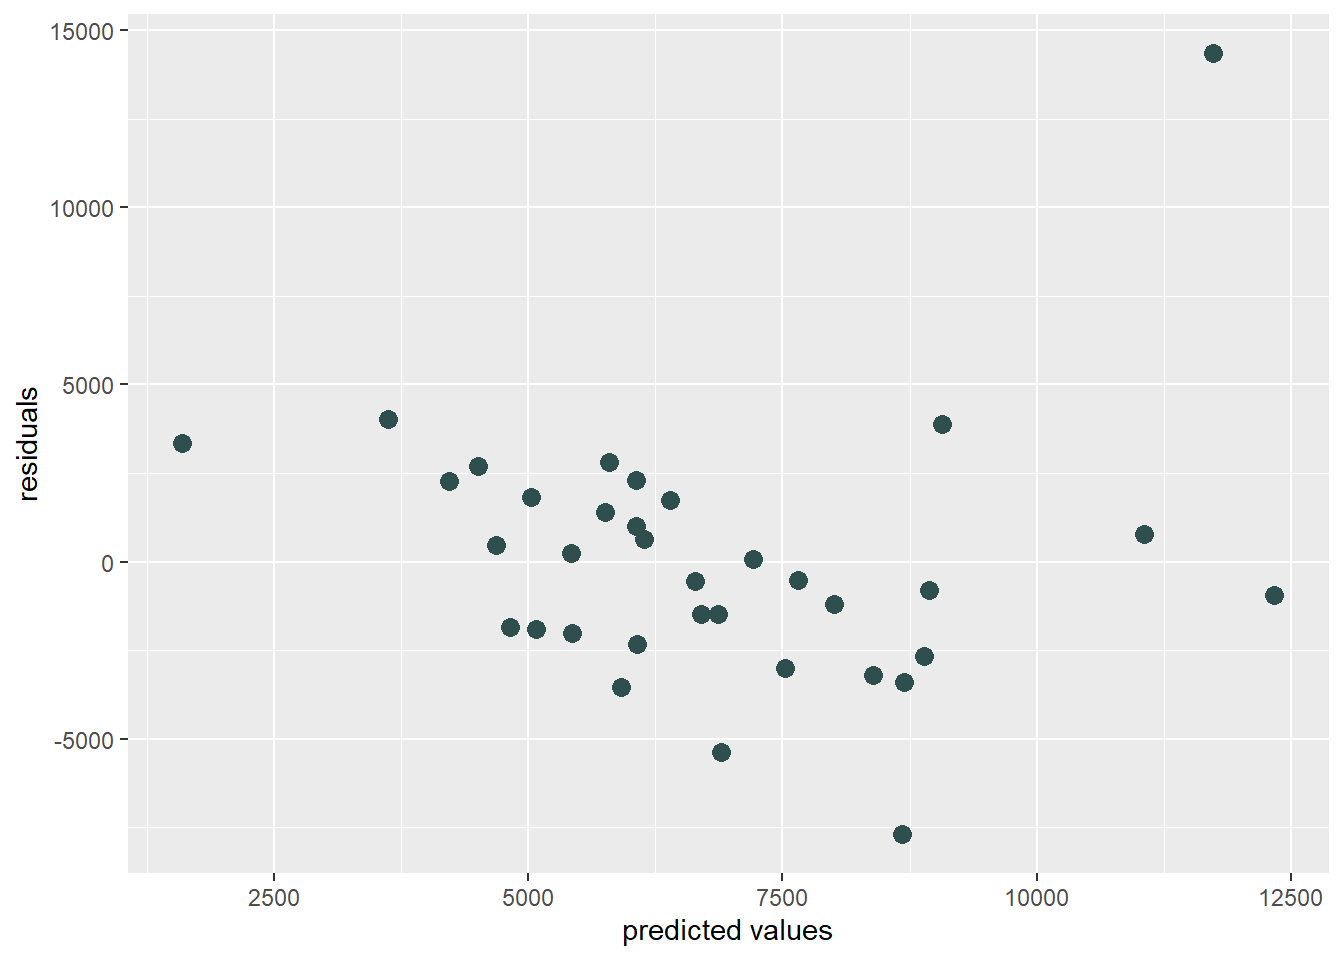
\includegraphics{Assignment-MSB104_files/figure-latex/unnamed-chunk-13-1.pdf}

\begin{verbatim}
## [1] 0.2157499
\end{verbatim}

\begin{verbatim}
##    Min. 1st Qu.  Median    Mean 3rd Qu.    Max. 
## 0.00000 0.03983 0.06158 0.08311 0.10279 0.29296
\end{verbatim}

\begin{Shaded}
\begin{Highlighting}[]
  \FunctionTok{ggplot}\NormalTok{(FR1, }\FunctionTok{aes}\NormalTok{(}\AttributeTok{x =}\NormalTok{ Year, }\AttributeTok{y=}\NormalTok{gini\_n3, }\AttributeTok{fill=}\NormalTok{id\_nuts2, }\AttributeTok{color=}\NormalTok{id\_nuts2)) }\SpecialCharTok{+}
  \FunctionTok{geom\_point}\NormalTok{(}\AttributeTok{lwd =}\NormalTok{ .}\DecValTok{8}\NormalTok{) }\SpecialCharTok{+}
   \FunctionTok{labs}\NormalTok{(}\AttributeTok{x =} \StringTok{"Year"}\NormalTok{, }\AttributeTok{y =} \StringTok{"GDP"}\NormalTok{)}
\end{Highlighting}
\end{Shaded}

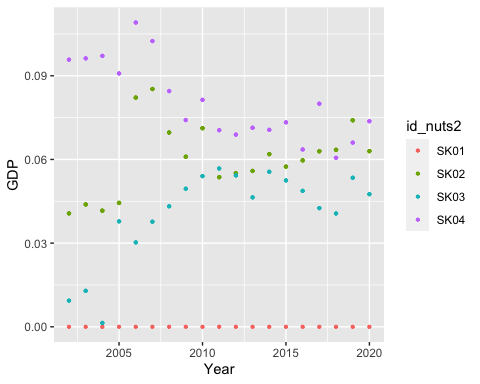
\includegraphics{Assignment-MSB104_files/figure-latex/unnamed-chunk-14-1.pdf}

\begin{verbatim}
## [1] 0.2851074
\end{verbatim}

\begin{verbatim}
##    Min. 1st Qu.  Median    Mean 3rd Qu.    Max. 
## 0.00000 0.04270 0.05866 0.05461 0.07195 0.12230
\end{verbatim}

\begin{Shaded}
\begin{Highlighting}[]
  \FunctionTok{ggplot}\NormalTok{(HU, }\FunctionTok{aes}\NormalTok{(}\AttributeTok{x =}\NormalTok{ Year, }\AttributeTok{y=}\NormalTok{gini\_n4, }\AttributeTok{fill=}\NormalTok{id\_nuts2, }\AttributeTok{color=}\NormalTok{id\_nuts2)) }\SpecialCharTok{+}
  \FunctionTok{geom\_point}\NormalTok{(}\AttributeTok{lwd =}\NormalTok{ .}\DecValTok{8}\NormalTok{) }\SpecialCharTok{+}
   \FunctionTok{labs}\NormalTok{(}\AttributeTok{x =} \StringTok{"Year"}\NormalTok{, }\AttributeTok{y =} \StringTok{"GDP"}\NormalTok{)}
\end{Highlighting}
\end{Shaded}

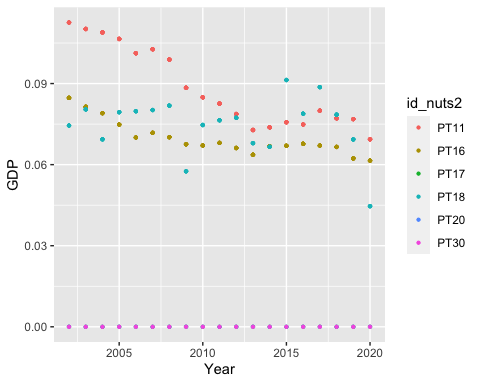
\includegraphics{Assignment-MSB104_files/figure-latex/unnamed-chunk-15-1.pdf}

\begin{verbatim}
## [1] 0.1619237
\end{verbatim}

\begin{verbatim}
##    Min. 1st Qu.  Median    Mean 3rd Qu.    Max. 
## 0.00000 0.06682 0.07380 0.06816 0.08043 0.11258
\end{verbatim}

\begin{Shaded}
\begin{Highlighting}[]
  \FunctionTok{ggplot}\NormalTok{(PT, }\FunctionTok{aes}\NormalTok{(}\AttributeTok{x =}\NormalTok{ Year, }\AttributeTok{y=}\NormalTok{gini\_n2, }\AttributeTok{fill=}\NormalTok{id\_nuts2, }\AttributeTok{color=}\NormalTok{id\_nuts2)) }\SpecialCharTok{+}
  \FunctionTok{geom\_point}\NormalTok{(}\AttributeTok{lwd =}\NormalTok{ .}\DecValTok{8}\NormalTok{) }\SpecialCharTok{+}
   \FunctionTok{labs}\NormalTok{(}\AttributeTok{x =} \StringTok{"Year"}\NormalTok{, }\AttributeTok{y =} \StringTok{"GDP"}\NormalTok{)}
\end{Highlighting}
\end{Shaded}

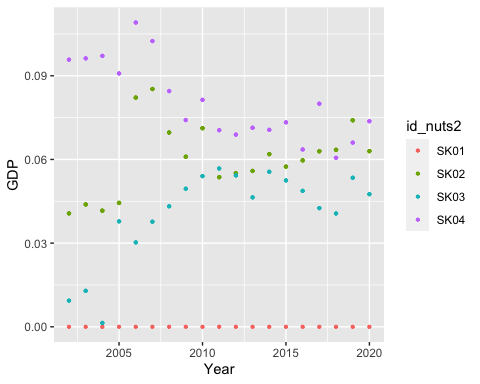
\includegraphics{Assignment-MSB104_files/figure-latex/unnamed-chunk-16-1.pdf}

\begin{verbatim}
## [1] 0.3026474
\end{verbatim}

\begin{verbatim}
##    Min. 1st Qu.  Median    Mean 3rd Qu.    Max. 
## 0.00000 0.04165 0.05632 0.05296 0.07075 0.10909
\end{verbatim}

\begin{Shaded}
\begin{Highlighting}[]
  \FunctionTok{ggplot}\NormalTok{(SK, }\FunctionTok{aes}\NormalTok{(}\AttributeTok{x =}\NormalTok{ Year, }\AttributeTok{y=}\NormalTok{gini\_n5, }\AttributeTok{fill=}\NormalTok{id\_nuts2, }\AttributeTok{color=}\NormalTok{id\_nuts2)) }\SpecialCharTok{+}
  \FunctionTok{geom\_point}\NormalTok{(}\AttributeTok{lwd =}\NormalTok{ .}\DecValTok{8}\NormalTok{) }\SpecialCharTok{+}
   \FunctionTok{labs}\NormalTok{(}\AttributeTok{x =} \StringTok{"Year"}\NormalTok{, }\AttributeTok{y =} \StringTok{"GDP"}\NormalTok{)}
\end{Highlighting}
\end{Shaded}

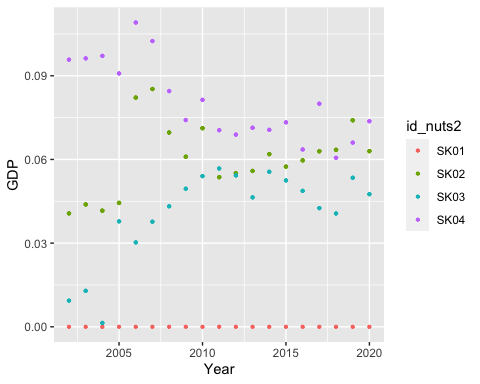
\includegraphics{Assignment-MSB104_files/figure-latex/unnamed-chunk-17-1.pdf}
Outliers

\begin{Shaded}
\begin{Highlighting}[]
\NormalTok{DKoutliers }\OtherTok{\textless{}{-}}\NormalTok{ DK }\SpecialCharTok{\%\textgreater{}\%}
  \FunctionTok{filter}\NormalTok{(gini\_n6}\SpecialCharTok{==}\DecValTok{0}\NormalTok{) }\SpecialCharTok{\%\textgreater{}\%}
  \FunctionTok{distinct}\NormalTok{(id\_nuts2)}
\NormalTok{DKoutliers}
\end{Highlighting}
\end{Shaded}

\begin{verbatim}
## # A tibble: 1 x 1
##   id_nuts2
##   <chr>   
## 1 DK05
\end{verbatim}

\begin{Shaded}
\begin{Highlighting}[]
\NormalTok{FRoutliers }\OtherTok{\textless{}{-}}\NormalTok{ FR1 }\SpecialCharTok{\%\textgreater{}\%}
  \FunctionTok{filter}\NormalTok{(gini\_n3}\SpecialCharTok{==}\DecValTok{0}\NormalTok{) }\SpecialCharTok{\%\textgreater{}\%}
  \FunctionTok{distinct}\NormalTok{(id\_nuts2)}
\NormalTok{FRoutliers}
\end{Highlighting}
\end{Shaded}

\begin{verbatim}
## # A tibble: 2 x 1
##   id_nuts2
##   <chr>   
## 1 FRD2    
## 2 FRE1
\end{verbatim}

\begin{Shaded}
\begin{Highlighting}[]
\NormalTok{HUoutliers }\OtherTok{\textless{}{-}}\NormalTok{ HU }\SpecialCharTok{\%\textgreater{}\%}
  \FunctionTok{filter}\NormalTok{(gini\_n4}\SpecialCharTok{==}\DecValTok{0}\NormalTok{) }\SpecialCharTok{\%\textgreater{}\%}
  \FunctionTok{distinct}\NormalTok{(id\_nuts2)}
\NormalTok{HUoutliers}
\end{Highlighting}
\end{Shaded}

\begin{verbatim}
## # A tibble: 2 x 1
##   id_nuts2
##   <chr>   
## 1 HU11    
## 2 HU12
\end{verbatim}

\begin{Shaded}
\begin{Highlighting}[]
\NormalTok{PToutliers }\OtherTok{\textless{}{-}}\NormalTok{ PT }\SpecialCharTok{\%\textgreater{}\%}
  \FunctionTok{filter}\NormalTok{(gini\_n2}\SpecialCharTok{==}\DecValTok{0}\NormalTok{) }\SpecialCharTok{\%\textgreater{}\%}
  \FunctionTok{distinct}\NormalTok{(id\_nuts2)}
\NormalTok{PToutliers}
\end{Highlighting}
\end{Shaded}

\begin{verbatim}
## # A tibble: 3 x 1
##   id_nuts2
##   <chr>   
## 1 PT17    
## 2 PT20    
## 3 PT30
\end{verbatim}

\begin{Shaded}
\begin{Highlighting}[]
\NormalTok{SKoutliers }\OtherTok{\textless{}{-}}\NormalTok{ SK }\SpecialCharTok{\%\textgreater{}\%}
  \FunctionTok{filter}\NormalTok{(gini\_n5}\SpecialCharTok{==}\DecValTok{0}\NormalTok{) }\SpecialCharTok{\%\textgreater{}\%}
  \FunctionTok{distinct}\NormalTok{(id\_nuts2)}
\NormalTok{SKoutliers}
\end{Highlighting}
\end{Shaded}

\begin{verbatim}
## # A tibble: 1 x 1
##   id_nuts2
##   <chr>   
## 1 SK01
\end{verbatim}

\hypertarget{discuss-briefly-if-there-are-noteworthy-outliers}{%
\section{Discuss briefly if there are noteworthy
outliers:}\label{discuss-briefly-if-there-are-noteworthy-outliers}}

What we have seen is that countries such as Denmark and Slovakia, which
do not have as many NUTS 3 regions, do not give us as much data. which
means that regions with low GDP will have a big impact.

When we removed the FRY countries in France, we did not get such big
differences as when we included them. We assume that this has something
to do with where these FRY regions are places in the world. France is a
large country with many NUTS 3 regions. which makes it easy to collect
data.

\hypertarget{assignment-2}{%
\subsection{Assignment 2}\label{assignment-2}}

At the second assigment we are looking at growth and inequity. We are
going to estimate the effete if regional development on regional
inequality, for the year 2010. Then we will disuse the goodness of fit
of our estimated model. We will plot the relationship between regional
development and regional inequality and the fitted line corresponding to
our estimate. We are also going to plot the residuals against the
predicted values of our model. There will be a discussion about the
classical assumptions OLS in light of our data and plots and other
determinants of inequity. We will also go back on Eurostat´s webpages
and download EurostatLinks to an external site. It will be for our
subset of countries regional (NUTS2, j) data related to transport
infrastructure, education and demographics. We are suppose to select on
variable per category that we would like to explore further in there
relationship to regional inequality. We will try to estimate a multiple
linear regression model with our new variables for 2010 and give a small
interpretation of our findings. In the end we will discuss the overall
fit of our model and the inference related to our findings.

\end{document}
